\documentclass[8pt,xcolor=table,dvipsnames]{beamer}
\usepackage{pgfpages}
\usepackage{yhmath}
\newcommand{\Mod}[1]{\ (\mathrm{mod}\ #1)}
\providecommand{\half}{\frac{1}{2}}
\newcommand{\dg}{^\circ}
\newcommand{\arc}[1]{\wideparen{#1}}
\usetheme{Madrid}

\title{Geometric Transformations II}
\subtitle{UMC K1, 2024}
\author{Nghia Doan}
\institute{MCC Club \& Competitions}
\date{\today}

\begin{document}

\begin{frame}[t]
    \frametitle{Geometric Transformations Lectures}
    \framesubtitle{Second Semester}
    \bigbreak
    Nghia Doan

    \bigbreak
    Math Club \& Competitions

    Victoria, BC, Canada
    \bigbreak
    \bigbreak
    (1) \textbf{January 5}: Geometric Transformations II: Translations. Half Turns. Sum of Half Turns.

    \bigbreak
    (2) \textbf{January 19}: Geometric Transformations III: Rotations by an Angle. Reflections over a Line.

    \bigbreak
    (3) \textbf{February 9}: Geometric Transformations IV: Homothety.
\end{frame}

\section{Translations}

\begin{frame}[t]
    \frametitle{Geometric Transformations II}
    \framesubtitle{Translation - Example 1}
    \begin{example}
        Given circles $\omega_1$, $\omega_2,$ and line $\ell.$
        \bigbreak
        Construct a segment $AB$ parallel with $\ell$ with a given length $AB=c$, such that $A \in \omega_1$ and $B \in \omega_2.$
    \end{example}
    \bigbreak
    \begin{center}
        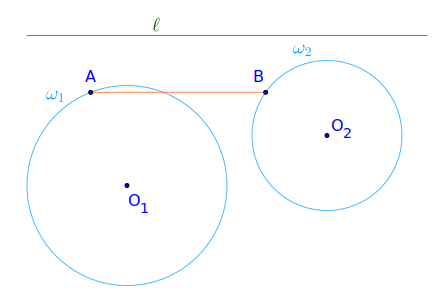
\includegraphics[width=6cm]{./svg/pdf/translation-5.pdf}
    \end{center}
\end{frame}

\begin{frame}[t]
    \frametitle{Geometric Transformations II}
    \framesubtitle{Translation - Example 1 - Solution}
    \textbf{Translate} the circle $\omega_1$ to $\omega'$ by a distance $O_1O' = c$ and $O_1O' \parallel \ell.$
    \bigbreak
    The intersections (if any) $\omega_2$ and $\omega'$ are $B$ and $B'$.
    \bigbreak
    They are the images of the translation of points $A$ and $A'$.
    Thus $AB = A'B' = c.$
    \begin{center}
        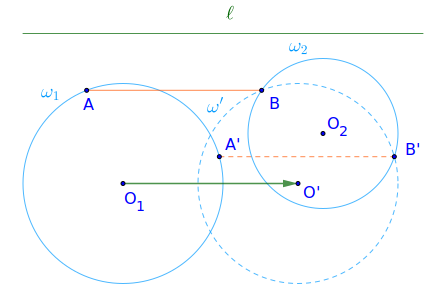
\includegraphics[width=6cm]{./svg/pdf/translation-5-1.pdf}
    \end{center}
\end{frame}

\begin{frame}[t]
    \frametitle{Geometric Transformations II}
    \framesubtitle{Translation - Example 2}
    \begin{example}
        $ABCD$ is a quadrilateral such that $AD = BC.$ $M$ and $N$ are midpoints of $AB$ and $CD$, respectively.
        \bigbreak
        $E$ is the intersection of (the extensions of) $AB$ and $CD.$
        \bigbreak
        Prove that $MN$ is parallel to the line $\ell,$ the angle bisector of $\angle AEB.$
    \end{example}
    \bigbreak
    \begin{center}
        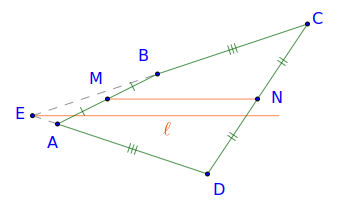
\includegraphics[width=6cm]{./svg/pdf/translation-4.pdf}
    \end{center}
\end{frame}

\begin{frame}[t]
    \frametitle{Geometric Transformations II}
    \framesubtitle{Translation - Example 2 - Solution}
    \textbf{Translate} $AD$ and $BC$ to $MM_1$ and $MM_2$, respectively.
    Then $DM_1$ and $CM_2$ are the images of $AM$ and $BM$ by the translation, thus $DM_1 \parallel CM_2$ and $DM_1 = CM_2$.
    Thus, $DM_1CM_2$ is a parallelogram.
    \bigbreak
    $\triangle NDM_1 \cong \triangle NCM_2$, thus $M_1, N, M_2$ are collinear. Therefore $NM_1 = NM_2.$
    \bigbreak
    $MM_1M_2$ is an isosceles triangle, thus the median $MN$ is the angle bisector, which is parallel to the angle bisector of $\angle AEB.$
    \begin{center}
        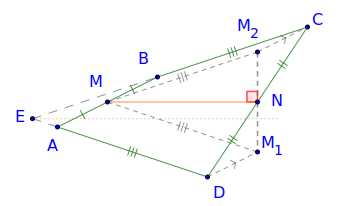
\includegraphics[width=6cm]{./svg/pdf/translation-4-1.pdf}
    \end{center}
\end{frame}

\begin{frame}[t]
    \frametitle{Geometric Transformations}
    \framesubtitle{Translation - Example 3}
    \begin{example}
        The point $O$ is situated inside the parallelogram $ABCD$ such that $\angle AOB+\angle COD=180^{\circ}$.
        Prove that $\angle OBC=\angle ODC$.
    \end{example}

    \bigbreak
    \begin{center}
        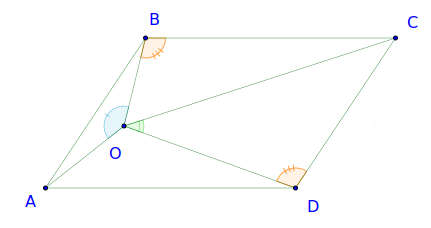
\includegraphics[width=8cm]{./svg/pdf/canada-mo-1997-4-0.pdf}
    \end{center}
\end{frame}

\begin{frame}[t]
    \frametitle{Geometric Transformations}
    \framesubtitle{Translation - Example 3 - Solution}
    \begin{center}
        \begin{overprint}
            \onslide<1>\centering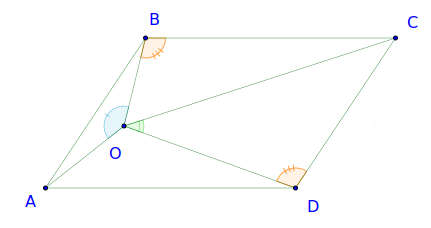
\includegraphics[width=8cm]{./svg/pdf/canada-mo-1997-4-0.pdf}
            \onslide<2->\centering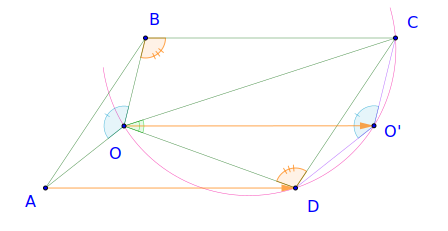
\includegraphics[width=8cm]{./svg/pdf/canada-mo-1997-4-1.pdf}
        \end{overprint}        
    \end{center}
    \onslide<2->{The translation by $\overrightarrow{AD}$ maps $A$ to $D$, $B$ to $C$, and $O$ to $O'$.}

    \bigbreak
    \onslide<3->{$ABCD$ is a parallelogram, $AD \parallel BC, AD = BC.$
    By the translation, $OO' \parallel AD, OO' = AD,$ thus $OO' \parallel BC, OO' = BC.$ 
    Therefore $OBCO'$ is a parallelogram. It implies that $\angle OBC = \angle OO'C.$}

    \bigbreak
    \onslide<4->{Since $\angle AOB+\angle COD=180^{\circ}$, so $\angle DO'C + \angle COD = 180\dg,$ or $CODO'$ is cyclic.
    Therefore $\angle ODC = \angle OO'C.$ Hence, $\boxed{\angle OBC = \angle ODC.}$}
\end{frame}

\section{Half Turns}

\begin{frame}[t]
    \frametitle{Geometric Transformations II}
    \framesubtitle{Half Turns - Example 1}
    \begin{example}
        Construct a line through $A$ intersecting line $\ell$ and circle $\omega$ at $P$ and $Q$, respectively,
        such that $AP = AQ.$
    \end{example}
    \bigbreak
    \begin{center}
        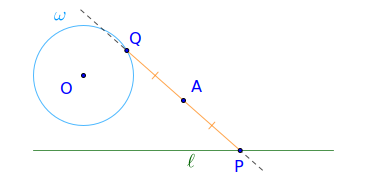
\includegraphics[width=6cm]{./svg/pdf/rotation-p8a.pdf}
    \end{center}
\end{frame}

\begin{frame}[t]
    \frametitle{Geometric Transformations II}
    \framesubtitle{Half Turns - Example 1 - Solution}
    Rotate the line $\ell$ half turn around $A$.
    Assume that $\ell'$, the image of $\ell$, intersects $\omega$ at $Q$.
    Draw a line through $A, Q$ intersects $\ell$ at $P$, then:
    \[
        \frac{1}{2}\ \text{turn}: P \rightarrow Q.
    \]

    \bigbreak
    We have: (1) $P$ is on $\ell$, (2) $Q$ is on $\omega$ ($\cap \ell'$), (3) $A, P,$ $Q$ are collinear, and 
    (4) $AP = AQ$.

    \begin{center}
        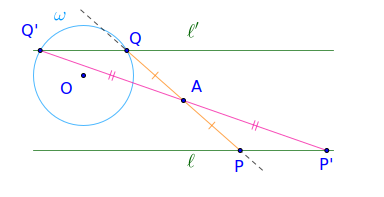
\includegraphics[width=6cm]{./svg/pdf/rotation-p8b.pdf}
    \end{center}

    We have \textbf{at most two solutions} (why?)
\end{frame}

\begin{frame}[t]
    \frametitle{Geometric Transformations II}
    \framesubtitle{Half Turns - Example 2}
    \begin{example}
        $P$ is an intersection point of circles $\omega_1$ and $\omega_2$.
        Construct a line through $P$ intersecting $\omega_1$ and $\omega_2$ at $A$ and $B$, respectively,
        such that $AP = PB.$
    \end{example}

    \bigbreak
    \begin{center}
        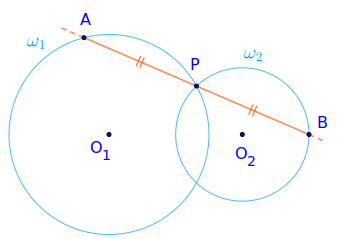
\includegraphics[width=5cm]{./svg/pdf/rotation-1a.pdf}
    \end{center}
\end{frame}

\begin{frame}[t]
    \frametitle{Geometric Transformations II}
    \framesubtitle{Half Turns - Example 2 - Solution}
    \begin{overprint}
        \onslide<1>Let \textbf{rotate} $\omega_2$ \textbf{half turn} ($180\dg$) around (or reflect $\omega_2$ over point) $P$.
        \bigbreak
        Let $A$ be the other intersection of $\omega_1$ and the image of $\omega_1$ (the dotted circle)
        and $B$ be the intersection of $AP$ with $\omega_2,$ then:
        \[
            \frac{1}{2}\ \text{turn}: B \rightarrow A.
        \]
        \bigbreak
        We have: (1) $A$ is on $\omega_1$ ($\cap\ \omega_2'$), (2) $B$ is on $\omega_2$, (3) $P, A,$ $B$ are collinear,
        and (4) $AP = PB$.
        \onslide<2>How many solutions?
        \begin{enumerate}
            \item If $|\omega_1 \cup \omega_2| = 2,$ then we have 1 solution.
            \item If $|\omega_1 \cup \omega_2| = 1,$ then we have no solution (why?)
            \item If $|\omega_1 \cup \omega_2| = 0,$ and the two radii are the same then we have infinitely many solutions
            otherwise no solution (why?).
        \end{enumerate}
    \end{overprint}    
    \begin{center}
        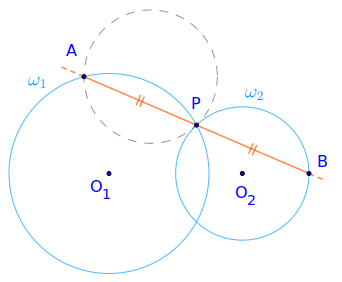
\includegraphics[width=5cm]{./svg/pdf/rotation-1b.pdf}
    \end{center}
\end{frame}

\begin{frame}[t]
    \frametitle{Geometric Transformations II}
    \framesubtitle{Half Turns - Example 3}
    \begin{example}
        $P$ is an intersection point of circles $\omega_1$ and $\omega_2$.
        Construct a line through $P$ intersecting $\omega_1$ and $\omega_2$ at $A$ and $B$, respectively,
        such that $AP = 2PB.$
    \end{example}

    \begin{center}
        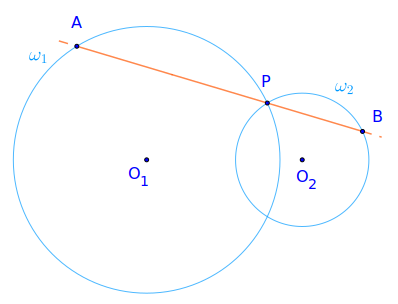
\includegraphics[width=5cm]{./svg/pdf/rotation-2a.pdf}
    \end{center}
\end{frame}

\begin{frame}[t]
    \frametitle{Geometric Transformations II}
    \framesubtitle{Half Turns - Example 3 - Solution}
    If \textbf{$M$ is the midpoint of $AP$, then $\angle OMP = 90\dg$ and $MP = PB$}.
    Thus $M$ is the intersection of $\omega_2'$, the image of $\omega_2$, and the circle $\gamma$ diameter $O_1P.$
    \begin{center}
        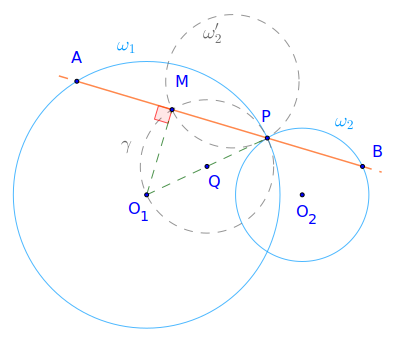
\includegraphics[width=5cm]{./svg/pdf/rotation-2b.pdf}
    \end{center}
    Thus we rotate $\omega_2$ \textbf{half turn} about $P$.
    Then we draw the circle $\gamma$ diameter $O_1P.$
    Their intersection is $M$. Line through $MP$ intersects $\omega_1$ and $\omega_2$ at $A$ and $B$ respectively.
    \[
        AM \stackrel{OM \perp MP}{=} MP \stackrel{B \rightarrow M}{=} PB \Rightarrow AP = 2PB.
    \]
\end{frame}

\begin{frame}[t]
    \frametitle{Geometric Transformations II}
    \framesubtitle{Half Turns - Example 4}
    \begin{example}
        $AB$ and $CD$ are chords of circle $\omega$. $J$ is a point on $CD$. Find point $X$ on the circumference of $\omega$ such that $JG = JF,$
        where $G$ and $F$ are intersections of $CD$ with $XA$ and $XB$, respectively.
    \end{example}

    \begin{center}
        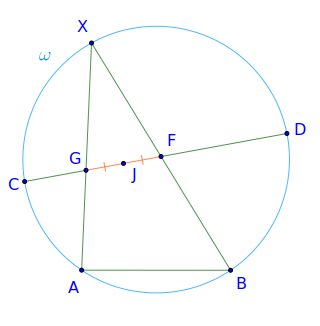
\includegraphics[width=5cm]{./svg/pdf/rotation-3a.pdf}
    \end{center}
\end{frame}

\begin{frame}[t]
    \frametitle{Geometric Transformations II}
    \framesubtitle{Half Turns - Example 4 - Solution}
    \begin{overprint}
        \onslide<1>The condition $GJ=JF$ give us the idea to rotate $X$ \textbf{half turn} about $J$ to $X'$.
        
        \bigbreak
        $\triangle XGJ \cong \triangle XFJ$ shows that $\angle XGJ = \angle JFX,$ thus $FX' \parallel XA.$
        Or $\angle X'FB = \angle AXB = \arc{AB}.$
        \begin{center}
            \includegraphics[width=5cm]{./svg/pdf/rotation-3b.pdf}
        \end{center}
        \onslide<2>We rotate $A$ \textbf{half turn} about $I$ to $A'$.
        Therefore, $AXA'X'$ is a parallelogram.
        \begin{center}
            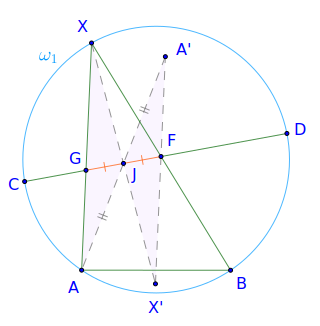
\includegraphics[width=5cm]{./svg/pdf/rotation-3c.pdf}
        \end{center}
        \onslide<3>$A'X'\parallel XA$ thus $X, F, A'$ are collinear.
        \begin{center}
            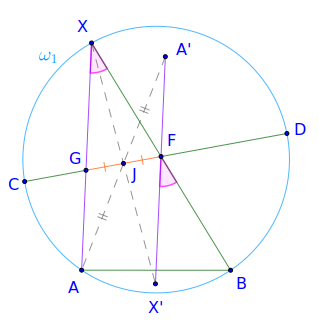
\includegraphics[width=5cm]{./svg/pdf/rotation-3d.pdf}
        \end{center}
        \onslide<4>$\angle A'FB = 180\dg - \angle F'XB = 180\dg - \angle AXB = 180\dg - \half \arc{AB}.$
        \bigbreak
        Hence, we first construct $A'$, then $F$ is the intersection the arc $\arc{A'B}$ with measure $180\dg - \half \arc{AB}$
        (how to construct an arc knowing the measure of the angle subtending it?) with the chord $CD.$
        \bigbreak
        Finally $X$ is the intersection of $BF$ with $\omega.$
        \begin{center}
            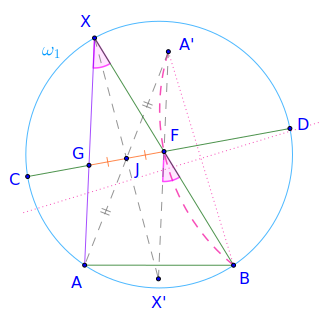
\includegraphics[width=5cm]{./svg/pdf/rotation-3e.pdf}
        \end{center}
    \end{overprint}
\end{frame}

\begin{frame}[t]
    \frametitle{Geometric Transformations II}
    \framesubtitle{Half Turns - Example 5}
    \begin{example}
        The strip formed by two parallel lines clearly has infinitely many centers of symmetry.
        Can a figure have more than one, but only a finite number of centers of symmetry (for example, can it have two and only two centers of symmetry)?
    \end{example}

    \begin{center}
        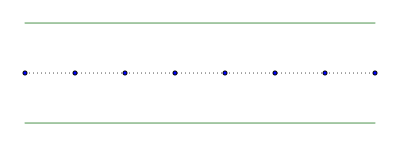
\includegraphics[width=5cm]{./svg/pdf/rotation-9.pdf}
    \end{center}
\end{frame}

\begin{frame}[t]
    \frametitle{Geometric Transformations II}
    \framesubtitle{Half Turns - Example 5 - Solution}
    \begin{overprint}
        \onslide<1>Assume that the figure $\mathcal{F}$ has two centers of symmetry, $O_1$ and $O_2$.

        \bigbreak
        Then the point $O_3$, obtained from $O_1$ by a half turn about $O_2$ is also a center of symmetry of $\mathcal{F}$.

        \bigbreak
        Indeed, if $A$ is any point of $\mathcal{F}$, then the points $A_1$, $A_2$, and $A'$, where $A_1$ is obtained from $A$ by a half turn about $O_2$,
        $A_2$ from $A_1$ by a half turn about $O_1$, and $A'$ from $A_2$ by a half turn about $O_2$, will also be points of $\mathcal{F}$
        (since $O_1$ and $O_2$ are centers of symmetry).
        \onslide<2>But the point $A'$ is also obtained from $A$ by a half turn about $O_3$!

        \bigbreak
        Indeed, the segments $AO_3$ and $O_3A'$ are equal, parallel, and have opposite directions,
        since the pairs of segments ($AO_3$, $A_1O_1$), ($A_1O_1$, $A_2O_1$), ($A_2O_1$, $A'O_3$) are equal, parallel, and have opposite directions.
    
        \bigbreak
        Thus if $A$ is any point of $\mathcal{F}$, then the symmetric point $A'$ obtained from $A$ by a half turn about $O_3$ is also a point of $\mathcal{F}$,
        that is, $O_3$ is a center of symmetry of $\mathcal{F}$.
        \onslide<3>Similarly one shows that the point $O_4$ , obtained from $O_2$ by a half turn about $O_3$, and the point $O_5$,
        obtained from $O_3$ by a half turn about $O_4$, etc. are centers of symmetry. 
        
        \bigbreak
        Thus we see that if the figure $\mathcal{F}$ has two distinct centers of symmetry then it has infinitely many.

        \bigbreak
        Now you can solve problem like this one \textbf{Prove that any circle has a single center!}
    \end{overprint}
    \begin{center}
        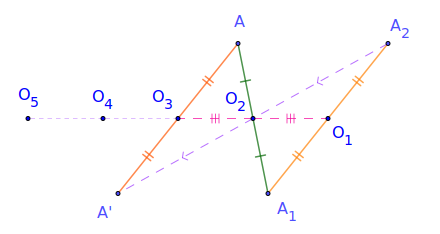
\includegraphics[width=8cm]{./svg/pdf/rotation-9b.pdf}
    \end{center}
\end{frame}

\section{Sum of Half Turns}

\begin{frame}[t]
    \frametitle{Geometric Transformations II}
    \framesubtitle{Sum of Half Turns - Example 1}
    \begin{example}
        $n$ is a positive integer. Let $O_1, O_2, \ldots, O_{2n}$ be points on the plane and $AB$ is an arbitrary segment.
        Let segment $A_1B_1$ be obtained from $AB$ by half turn about $O_1$, let $A_2B_2$ be obtained from $A_1B_1$ by half turn about $O_2$, $\ldots,$
        and finally let $A_{2n}B_{2n}$ be obtained from $A_{2n-1}B_{2n-1}$ by half turn about $O_{2n}$ (see the figure for $n=2.$)

        \bigbreak
        Show that $AA_{2n} = BB_{2n}.$
    \end{example}

    \begin{center}
        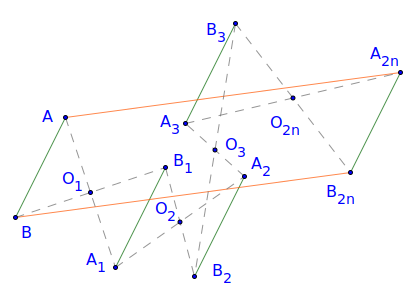
\includegraphics[width=5cm]{./svg/pdf/translation-1.pdf}
    \end{center}
\end{frame}

\begin{frame}[t]
    \frametitle{Geometric Transformations II}
    \framesubtitle{Sum of Half Turns - Example 1 - Solution}
    \begin{overprint}
        \onslide<1>First, it is easy to see that \textbf{the sum of two half turns} around $O_1$ and $O_2$ is \textbf{a translation}:
        \[ 
            AA_2 \parallel BB_2 \parallel O_1O_2 \quad \text{and} \quad AA_2 = BB_2 = 2O_1O_2.
        \]
        \begin{center}
            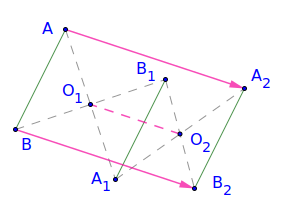
\includegraphics[width=5cm]{./svg/pdf/translation-1b.pdf}
        \end{center}
        \onslide<2>Thus, for an \textbf{even $2n$ number of translations}, their sum is just \textbf{another translation}, hence
        \[
            AA_{2n} = BB_{2n}.
        \]
        \begin{center}
            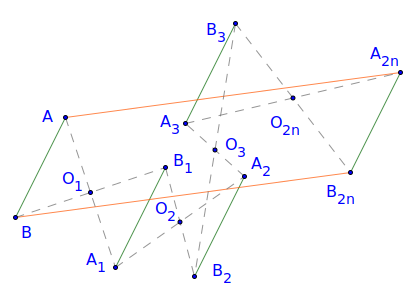
\includegraphics[width=5cm]{./svg/pdf/translation-1.pdf}
        \end{center}
    
        \bigbreak
        Is the conclusion still true if we have an \textbf{odd number of translations}? Why or why not?        
    \end{overprint}
\end{frame}

\begin{frame}[t]
    \frametitle{Geometric Transformations II}
    \framesubtitle{Sum of Half Turns - Example 2}
    \begin{example}
        $n$ is a positive odd integer. Let $O_1, O_2, \ldots, O_{n}$ be points on the plane.
        Let an arbitrary point $A$ be moved successively by half turns about $O_1, O_2, \ldots, O_{n}$
        and then once again moved successively by half turns about the same points $O_1, O_2, \ldots, O_{n}$.
        
        \bigbreak
        Show that the point $A_{2n}$, obtained as the result of these $2n$ half turns, coincides with the point $A.$
    \end{example}

    \begin{center}
        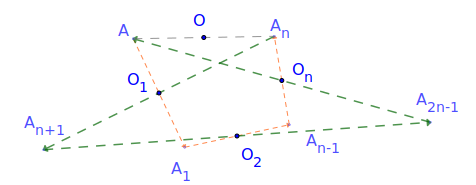
\includegraphics[width=5cm]{./svg/pdf/translation-2a.pdf}
    \end{center}
\end{frame}

\begin{frame}[t]
    \frametitle{Geometric Transformations II}
    \framesubtitle{Sum of Half Turns - Example 2 - Solution}
    \onslide<1->Since the \textbf{sum of an odd number of half turns} is \textbf{a half turn}, the point $A_n$, obtained from $A$ by the $n$
    successive half turns about the points $O_1, O_2, \ldots, O_{n}$ can also be obtained from $A$ by a single half turn about some point $O$.
    \begin{center}
        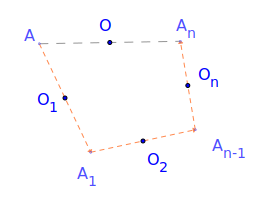
\includegraphics[width=2.8cm]{./svg/pdf/translation-2b.pdf}
        \qquad \qquad
        \onslide<2->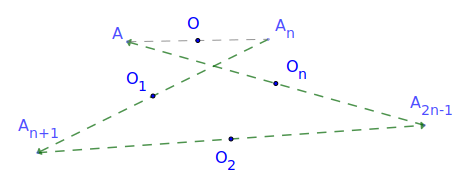
\includegraphics[width=6cm]{./svg/pdf/translation-2d.pdf}
    \end{center}
    \onslide<2->It is important to note that \textbf{$O$ depends on $O_1, O_2, \ldots, O_{n}$ only} and not $A$.
    \onslide<3>\begin{center}
        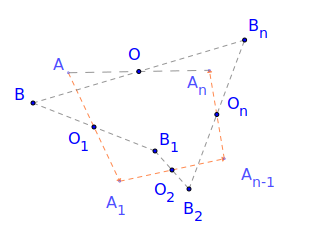
\includegraphics[width=4.3cm]{./svg/pdf/translation-2c.pdf}
    \end{center}
    The point $A_{2n}$ is obtained from $A_n$, by these same $n$ half turns;
    therefore it can also be obtained from $A_n$, by the single half turn about the point $O$.
    But this means that $A_{2n}$, coincides with $A$, because of the two half turns around the same point $O$.
    
    Is the conclusion still true if we have $n$ as \textbf{even number}? Why or why not?
\end{frame}

\begin{frame}[t]
    \frametitle{Geometric Transformations II}
    \framesubtitle{Sum of Half Turns - Example 3}
    \begin{example}
        $A_1A_2 \ldots A_{2n}$ is a $2n-$gon. $M_1, M_2, \ldots, M_{2n}$ are the midpoints of $A_1A_2,$ $A_2A_3,\ \ldots,$ $A_{2n}A_1$, respectively.
        Prove that there exists a $n-$gon whose sides are equal and parallel to the segments $M_1M_2,$ $M_3M_4,$ $\ldots$, $M_{2n-1}M_{2n}$
        and there exists a $n-$gon whose sides are equal and parallel to the segments $M_2M_3,$ $\ldots$, $M_{2n-2}M_{2n-1}$, $M_{2n}M_1.$ 
    \end{example}

    \begin{center}
        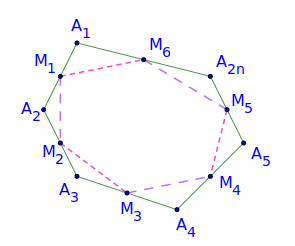
\includegraphics[width=5cm]{./svg/pdf/translation-3a.pdf}
    \end{center}
\end{frame}

\begin{frame}[t]
    \frametitle{Geometric Transformations II}
    \framesubtitle{Sum of Half Turns - Example 3 - Solution}
    Note that by $2n$ half turns around $M_1, M_2, \ldots, M_{2n}$:
    \[
        A_1 \rightarrow A_2 \rightarrow A_3 \rightarrow  \cdots \rightarrow  A_{2n} \rightarrow A_1.
    \]
    
    The sum of two half turns around $M_1$ and $M_2$ is a translation $A_1 \rightarrow A_3$ with distance $A_1A_3 = 2 M_1M_2$
    similarly the sum of two half turns around $M_3$ and $M_4$ is a translation $A_3 \rightarrow A_5$ with distance $A_3A_4 = 2 M_3M_4$
    and so on.

    \begin{center}
        \includegraphics[width=5cm]{./svg/pdf/translation-3b.pdf}
    \end{center}

    Furthermore after $n$ translations: $A_1 \rightarrow A_1,$ therefore the sum of them is an \textbf{identity transformation},
    thus \textbf{the $n$ translations} form a \textbf{close path} and therefore is an $n-$gon.

    \bigbreak
    Hence, each of the sides is equal and parallel to the segments $M_1M_2,$ $M_3M_4,$ $\ldots$, $M_{2n-1}M_{2n}$.
\end{frame}

\begin{frame}[t]
    \frametitle{Geometric Transformations II}
    \framesubtitle{IMO 2005 SL}
    \begin{example}
        Given a triangle $ABC$ satisfying $AB+BC=3 AC$.
        The incircle of triangle $ABC$ has center $I$ and touches the sides $AB$ and $BC$ at the points $D$ and $E$, respectively.
        Let $K$ and $L$ be the reflections of the points $D$ and $E$ with respect to $I$.
        \bigbreak
        Prove that the points $A$, $C$, $K$, $L$ lie on one circle.
    \end{example}

    \begin{center}
        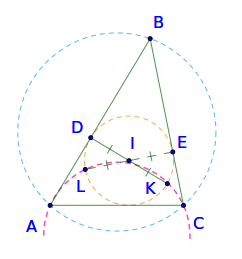
\includegraphics[width=4cm]{./svg/pdf/imo-sl-2005-g1.pdf}
    \end{center}
\end{frame}

\begin{frame}[t]
    \frametitle{Geometric Transformations II}
    \framesubtitle{IMO 2005 SL - Solution}
    \begin{overprint}
        \onslide<1>What do we have?
        \[ 
            AB+BC=3AC \Rightarrow \half(AB+BC-CA) = CA.
        \]
        This means that the tangent segment $BD$ and $BE$ is equal to $CA$!
        \bigbreak
        Let $P$ be the other intersection of $B$ with $(ABC).$ Let $M$ be the midpoint of $AC,$ then:
        \[
            BD = AC = 2MC,\ \angle DBI = \angle MCP \Rightarrow \triangle DBI \sim \triangle MCP\ \text{with similarity ratio}\ 2.
        \]
        \begin{center}
            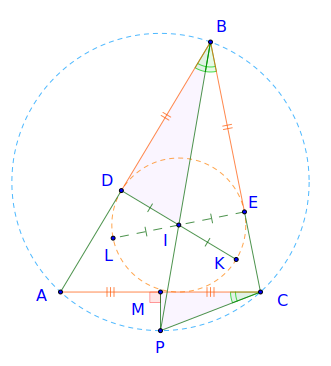
\includegraphics[width=4cm]{./svg/pdf/imo-sl-2005-g1-2.pdf}
        \end{center}
        \onslide<2>Let $N$ be the foot of the altitude from $P$ to $IK$. Now:
        \[
            PI = PC\ (= PA)\ \text{(why?)}\ \text{and}\ \angle NIP = \angle DIB \Rightarrow \triangle PNI \cong \triangle CMP.
        \]
        Thus,
        \[
            \triangle DBI \sim \triangle NPI\ \text{with similarity ratio}\ 2.
        \]
        \begin{center}
            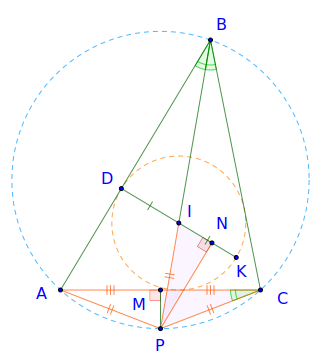
\includegraphics[width=4cm]{./svg/pdf/imo-sl-2005-g1-3.pdf}
        \end{center}
        \onslide<3>Now, by comparing corresponding segments: $DI, NI$:
        \[
            DI = 2 NI \Rightarrow KI = 2 NI \Rightarrow \triangle IPK\ \text{isosceles} \Rightarrow PK = PI,\ \text{similarly}\ PL = PA.
        \]
        Thus \[ PC = PK = PI = PL = PA. \]
        \begin{center}
            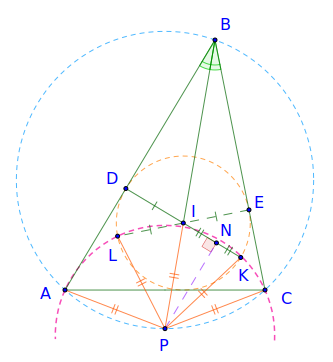
\includegraphics[width=4cm]{./svg/pdf/imo-sl-2005-g1-4.pdf}
        \end{center}
    \end{overprint}
\end{frame}

\end{document}
